%----------------------------------------------------------------------------------------
%
% A LaTeX-template for 1DV510. Modified and translated by Björn Lindenberg at LNU.
% Based on an original master thesis template created by Marcus Wilhelmsson at LNU.
%
%----------------------------------------------------------------------------------------

% Settings and document configuration

\documentclass[a4paper,12pt]{article} 
\usepackage[T1]{fontenc} 
\usepackage{times} 
\usepackage[swedish,english]{babel} 
\usepackage[utf8]{inputenc} 
\usepackage{dtk-logos} 
\usepackage{wallpaper} 
\usepackage[absolute]{textpos} 
\usepackage[top=2cm, bottom=2.5cm, left=3cm, right=3cm]{geometry} 
\usepackage[parfill]{parskip} 
\usepackage{csquotes} 
\usepackage{float} 
\usepackage{lipsum} % Used for dummy text. Can be removed.
\usepackage{listings, color}

\lstdefinestyle{Asm}{
  belowcaptionskip=1\baselineskip,
  breaklines=true,
  frame=L,
  xleftmargin=\parindent,
  language=[x86masm]Assembler,
  showstringspaces=false,
  basicstyle=\footnotesize\ttfamily,
  keywordstyle=\bfseries\color{purple!40!black},
  commentstyle=\itshape\color{green!40!black},
  identifierstyle=\color{blue},
  stringstyle=\color{orange},
}

% Fontsizes for section headings.
\usepackage{sectsty} 
\sectionfont{\fontsize{14}{15}\selectfont}
\subsectionfont{\fontsize{12}{15}\selectfont}
\subsubsectionfont{\fontsize{12}{15}\selectfont}

%----------------------------------------------------------------------------------------
%	This part is used for the text box on the title page
%----------------------------------------------------------------------------------------
\newsavebox{\mybox}
\newlength{\mydepth}
\newlength{\myheight}

\newenvironment{sidebar}%
{\begin{lrbox}{\mybox}\begin{minipage}{\textwidth}}%
{\end{minipage}\end{lrbox}%
 \settodepth{\mydepth}{\usebox{\mybox}}%
 \settoheight{\myheight}{\usebox{\mybox}}%
 \addtolength{\myheight}{\mydepth}%
 \noindent\makebox[0pt]{\hspace{-20pt}\rule[-\mydepth]{1pt}{\myheight}}%
 \usebox{\mybox}}

%----------------------------------------------------------------------------------------
%	Title
%----------------------------------------------------------------------------------------
\newcommand\BackgroundPic{
    \put(-2,-3){
    
\includegraphics[keepaspectratio,scale=0.3]{img/lnu_etch.png} % Background image
    }
}
\newcommand\BackgroundPicLogo{
    \put(30,740){
    
\includegraphics[keepaspectratio,scale=0.10]{img/logo.png} % LNU logo
    }
}

\title{
\vspace{-8cm}
\begin{sidebar}
    \vspace{10cm}
    \normalfont \normalsize
    \huge Computer Technology I\\ % Main title
    \vspace{-1.3cm}
\end{sidebar}
\vspace{3cm}
\begin{flushleft}
    \huge Lab. 5 :Display JHD202 % Subtitle
     \small \\ \emph{}
\end{flushleft}
\null
\vfill
\begin{textblock}{5}(10,13)
\begin{flushright}
\begin{minipage}{\textwidth}
\begin{flushleft} \large
\emph{Author:}\textsc{ Loic GALLAND, Leonardo PEDRO}\\  % Author
\emph{Supervisor:}  \textsc{} \\  % Author
\emph{Semester:} Autumn 2019\\ % Semester
\emph{Area:} Computer Science \\ % Area
\emph{Course code:} 1DT301 % Course
\end{flushleft}
\end{minipage}
\end{flushright}
\end{textblock}
}

\date{} % Empty date command. Use \today inside for today's date.
\author{} % Normally one would use this to define authors. However in this case the title command takes care of everything, so we leave the field empty to get rid of warnings. 

\begin{document}

\pagenumbering{gobble} % Turn off page numbering
\newgeometry{left=5cm}
\AddToShipoutPicture*{\BackgroundPic} % Adds the background image to the title page
\AddToShipoutPicture*{\BackgroundPicLogo} % Adds the logo to the title page
\maketitle % Prints the title
\restoregeometry
\clearpage

\pagenumbering{roman} % Roman page numbering for abstract page


\selectlanguage{english}

\newpage

\pagenumbering{gobble} % Turn off page numbering
\tableofcontents 

\newpage
\pagenumbering{arabic} % Turn on page numbering


\section{Task 1 -  Write a program that displays a character on the display}

\textit{Write a program in Assembly that displays the character "percent". Look in the data sheet how to initiate the display. The data sheet you’ll find on https://www.student.vxu.se/. The display will be connected as in the figure above. 4-bit-mode should be used, since only RS, E, D7, D6, D5 and D4 are connected to I/O-pins on the STK600.}

\lstset{style=Asm}
\begin{lstlisting}
;>>>>>>>>>>>>>>>>>>>>>>>>>>>>>>>>>>>>>>>>>>>>>>>>>>>>>>>>>>>
; 1DT301, Computer Technology I
; Date: 2019-10-11
; Author:
; Loic GALLAND
; Leonardo PEDRO
;
; Lab number: 5
; Title: Display JHD202
;
; Hardware: STK600, CPU ATmega2560
;
; Function: Program that shows a percentage sign on the display
;
; Input ports: No input ports
;
; Output ports: PORTE for the display
;
; Subroutines: If applicable.
; Included files: m2560def.inc
;<<<<<<<<<<<<<<<<<<<<<<<<<<<<<<<<<<<<<<<<<<<<<<<<<<<<<<<<<<<
.include 	"m2560def.inc"
.def	Temp	= r16
.def	Data	= r17
.def	RS	= r18

.equ	BITMODE4	= 0b00000010		; 4-bit operation
.equ	CLEAR	= 0b00000001			; Clear display
.equ	DISPCTRL	= 0b00001111		; Display on, cursor on, blink on.

.cseg
.org	0x0000				; Reset vector
	jmp reset

.org	0x0072

reset:	

	ldi Temp, HIGH(RAMEND)	; Temp = high byte of ramend address
	out SPH, Temp			; sph = Temp
	ldi Temp, LOW(RAMEND)	; Temp = low byte of ramend address
	out SPL, Temp			; spl = Temp

	ser Temp				; r16 = 0b11111111
	out DDRE, Temp			; port E = outputs ( Display JHD202A)
	clr Temp				; r16 = 0
	out PORTE, Temp	

; **
; ** init_display
; **
init_disp:	
	rcall power_up_wait		; wait for display to power up
	ldi Data, BITMODE4		; 4-bit operation
	rcall write_nibble		; (in 8-bit mode)
	rcall short_wait		; wait min. 39 us
	ldi Data, DISPCTRL		; disp. on, blink on, curs. On
	rcall write_cmd			; send command
	rcall short_wait		; wait min. 39 us

rcall clr_disp	
ldi Data, 0x25
rcall write_char
loop:	nop
	rjmp loop			; loop forever


clr_disp:	
	ldi Data, CLEAR			; clr display
	rcall write_cmd			; send command
	rcall long_wait			; wait min. 1.53 ms
	ret

; **
; ** write char/command
; **

write_char:		
	ldi RS, 0b00100000		; RS = high
	rjmp write
write_cmd: 	
	clr RS					; RS = low
write:	
	mov Temp, Data			; copy Data
	andi Data, 0b11110000	; mask out high nibble
	swap Data				; swap nibbles
	or Data, RS				; add register select
	rcall write_nibble		; send high nibble
	mov Data, Temp			; restore Data
	andi Data, 0b00001111	; mask out low nibble
	or Data, RS				; add register select

write_nibble:
	rcall switch_output		; Modify for display JHD202A, port E
	nop						; wait 542nS
	sbi PORTE, 5			; enable high, JHD202A
	nop
	nop						; wait 542nS
	cbi PORTE, 5			; enable low, JHD202A
	nop
	nop						; wait 542nS
	ret

; **
; ** busy_wait loop
; **
short_wait:	
	clr zh					; approx 50 us
	ldi zl, 30
	rjmp wait_loop
long_wait:	
	ldi zh, HIGH(1000)		; approx 2 ms
	ldi zl, LOW(1000)
	rjmp wait_loop
dbnc_wait:	
	ldi zh, HIGH(4600)		; approx 10 ms
	ldi zl, LOW(4600)
	rjmp wait_loop
power_up_wait:
	ldi zh, HIGH(9000)		; approx 20 ms
	ldi zl, LOW(9000)

wait_loop:	
	sbiw z, 1				; 2 cycles
	brne wait_loop			; 2 cycles
	ret

; **
; ** modify output signal to fit LCD JHD202A, connected to port E
; **

switch_output:
	push Temp
	clr Temp
	sbrc Data, 0				; D4 = 1?
	ori Temp, 0b00000100		; Set pin 2 
	sbrc Data, 1				; D5 = 1?
	ori Temp, 0b00001000		; Set pin 3 
	sbrc Data, 2				; D6 = 1?
	ori Temp, 0b00000001		; Set pin 0 
	sbrc Data, 3				; D7 = 1?
	ori Temp, 0b00000010		; Set pin 1 
	sbrc Data, 4				; E = 1?
	ori Temp, 0b00100000		; Set pin 5 
	sbrc Data, 5				; RS = 1?
	ori Temp, 0b10000000		; Set pin 7 (wrong in previous version)
	out porte, Temp
	pop Temp
	ret
\end{lstlisting}
\newpage
This is the flowchart of the task 1:
\begin{center}
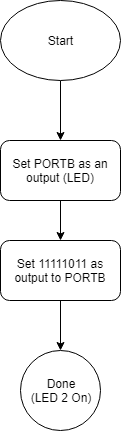
\includegraphics[scale=0.8]{img/Task1.png}
\end{center}
\newpage
\section{Task 2 - Electronic bingo machine}
\textit{You should create an electronic bingo generator. The generator should create random numbers between 1 and 75. The numbers should be displayed on the display. Clear the display before a new value is displayed. Use interrupt and a pushbutton for the input.}

\lstset{style=Asm}
\begin{lstlisting}
;>>>>>>>>>>>>>>>>>>>>>>>>>>>>>>>>>>>>>>>>>>>>>>>>>>>>>>>>>>>
; 1DT301, Computer Technology I
; Date: 2019-10-11
; Author:
; Loic GALLAND
; Leonardo PEDRO
;
; Lab number: 5
; Title: Display JHD202
;
; Hardware: STK600, CPU ATmega2560
;
; Function: Program that creates a bingo machine.
;
; Input ports: PORTD for the switches
;
; Output ports: PORTE for the display
;
; Subroutines: If applicable.
; Included files: m2560def.inc
;<<<<<<<<<<<<<<<<<<<<<<<<<<<<<<<<<<<<<<<<<<<<<<<<<<<<<<<<<<<
.include 	"m2560def.inc"
.def	Temp	= r16
.def	Data	= r17
.def	RS	= r18
.def	RandomNumber= r20
.def	RandomNumber2 = r21
.def	NumberBetween05= r22

.equ	BITMODE4	= 0b00000010		; 4-bit operation
.equ	CLEAR	= 0b00000001			; Clear display
.equ	DISPCTRL	= 0b00001111		; Display on, cursor on, blink on.


.cseg
.org	0x0000				; Reset vector
	jmp reset
.org Int0addr
rjmp interrupt

.org	0x0072

reset:	

	ldi Temp, HIGH(RAMEND)	; Temp = high byte of ramend address
	out SPH, Temp			; sph = Temp
	ldi Temp, LOW(RAMEND)	; Temp = low byte of ramend address
	out SPL, Temp			; spl = Temp

	ser Temp				; r16 = 0b11111111
	out DDRE, Temp			; port E = outputs ( Display JHD202A)
	clr Temp				; r16 = 0
	out PORTE, Temp	

	ldi Temp,0x00
	out DDRD,Temp


	ldi Temp,0b00000010 ;Setting INT0 into falling edge
	sts EICRA,Temp
	ldi Temp,0b0000001 ;Enable INT0
	out EIMSK,Temp
	ldi RandomNumber,0x31
	ldi RandomNumber2,0x30
	ldi NumberBetween05,0x30

	sei


; **
; ** init_display
; **
init_disp:	
	rcall power_up_wait		; wait for display to power up

	ldi Data, BITMODE4		; 4-bit operation
	rcall write_nibble		; (in 8-bit mode)
	rcall short_wait		; wait min. 39 us
	ldi Data, DISPCTRL		; disp. on, blink on, curs. On
	rcall write_cmd			; send command
	rcall short_wait		; wait min. 39 us

	


loop:	 
	rcall increaseNumber
	rcall increaseNumber2
	rcall increaseNumber3
rjmp loop			; loop forever


clr_disp:	
	ldi Data, CLEAR			; clr display
	rcall write_cmd			; send command
	rcall long_wait			; wait min. 1.53 ms
	ret

; **
; ** write char/command
; **

increaseNumber: ;To get the first digit 

	cpi RandomNumber,0x37 ; 
	breq ResetDisplay

	inc RandomNumber
	jmp END

	ResetDisplay:
		ldi RandomNumber,0x31
	END:
ret 

increaseNumber2:	;Second digit if the first is not 7
	cpi RandomNumber2,0x39 ; 
	breq ResetDisplay2

	inc RandomNumber2
	jmp END2

	ResetDisplay2:
		ldi RandomNumber2,0x30
	END2:
ret 

increaseNumber3: ;Second digit if the first is  7
	cpi NumberBetween05,0x35 ; 
	breq ResetDisplay3

	inc NumberBetween05
	jmp END3

	ResetDisplay3:
		ldi NumberBetween05,0x30
	END3:
ret 

write_char:		
	ldi RS, 0b00100000		; RS = high
	rjmp write
write_cmd: 	
	clr RS					; RS = low
write:	
	mov Temp, Data			; copy Data
	andi Data, 0b11110000	; mask out high nibble
	swap Data				; swap nibbles
	or Data, RS				; add register select
	rcall write_nibble		; send high nibble
	mov Data, Temp			; restore Data
	andi Data, 0b00001111	; mask out low nibble
	or Data, RS				; add register select

write_nibble:
	rcall switch_output		; Modify for display JHD202A, port E
	nop						; wait 542nS
	sbi PORTE, 5			; enable high, JHD202A
	nop
	nop						; wait 542nS
	cbi PORTE, 5			; enable low, JHD202A
	nop
	nop						; wait 542nS
	ret

; **
; ** busy_wait loop
; **
short_wait:	
	clr zh					; approx 50 us
	ldi zl, 30
	rjmp wait_loop
long_wait:	
	ldi zh, HIGH(1000)		; approx 2 ms
	ldi zl, LOW(1000)
	rjmp wait_loop
dbnc_wait:	
	ldi zh, HIGH(4600)		; approx 10 ms
	ldi zl, LOW(4600)
	rjmp wait_loop
power_up_wait:
	ldi zh, HIGH(9000)		; approx 20 ms
	ldi zl, LOW(9000)

wait_loop:	
	sbiw z, 1				; 2 cycles
	brne wait_loop			; 2 cycles
	ret

; **
; ** modify output signal to fit LCD JHD202A, connected to port E
; **

switch_output:
	push Temp
	clr Temp
	sbrc Data, 0				; D4 = 1?
	ori Temp, 0b00000100		; Set pin 2 
	sbrc Data, 1				; D5 = 1?
	ori Temp, 0b00001000		; Set pin 3 
	sbrc Data, 2				; D6 = 1?
	ori Temp, 0b00000001		; Set pin 0 
	sbrc Data, 3				; D7 = 1?
	ori Temp, 0b00000010		; Set pin 1 
	sbrc Data, 4				; E = 1?
	ori Temp, 0b00100000		; Set pin 5 
	sbrc Data, 5				; RS = 1?
	ori Temp, 0b10000000		; Set pin 7 (wrong in previous version)
	out porte, Temp
	pop Temp
	ret

interrupt: 	;USART Interrupt
	rcall clr_disp
	mov Data, RandomNumber
	rcall write_char
	call power_up_wait
	cpi RandomNumber,0x37
	brlt IfLessSeven

	call power_up_wait
	mov Data, NumberBetween05
	rcall write_char
	rjmp endInt

	IfLessSeven:
		call power_up_wait
		mov Data, RandomNumber2
		rcall write_char

endInt:

RETI 
\end{lstlisting}
\newpage
This is the flowcharts of the task 2:
\begin{center}
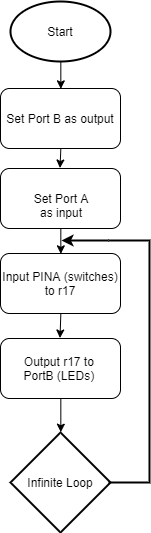
\includegraphics[scale=0.9]{img/Task2.png}
\end{center}
\begin{center}
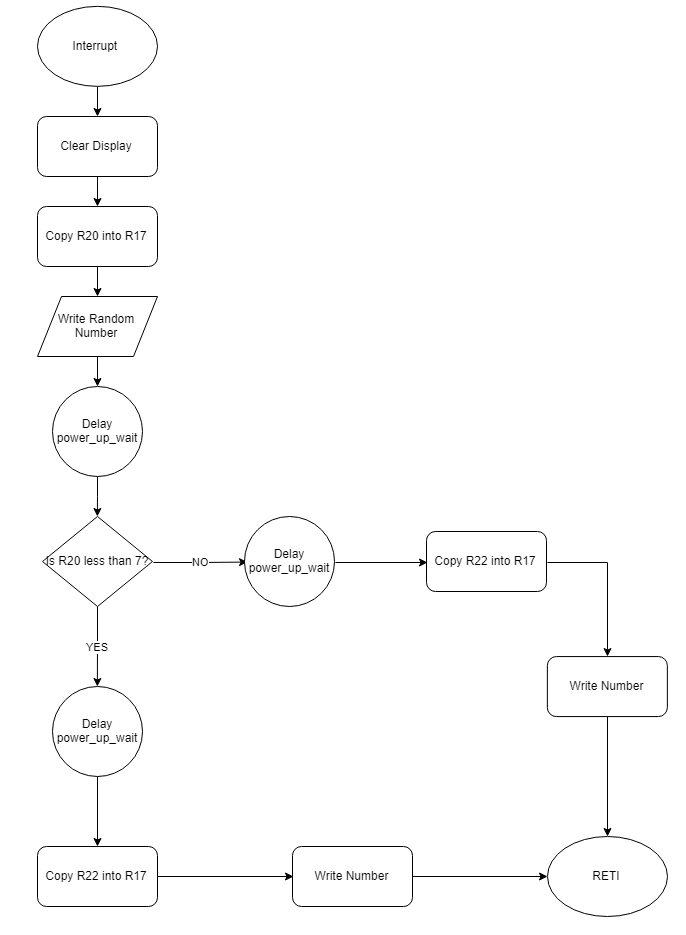
\includegraphics[scale=1.1]{img/Task2-2.png}
\end{center}
\begin{center}
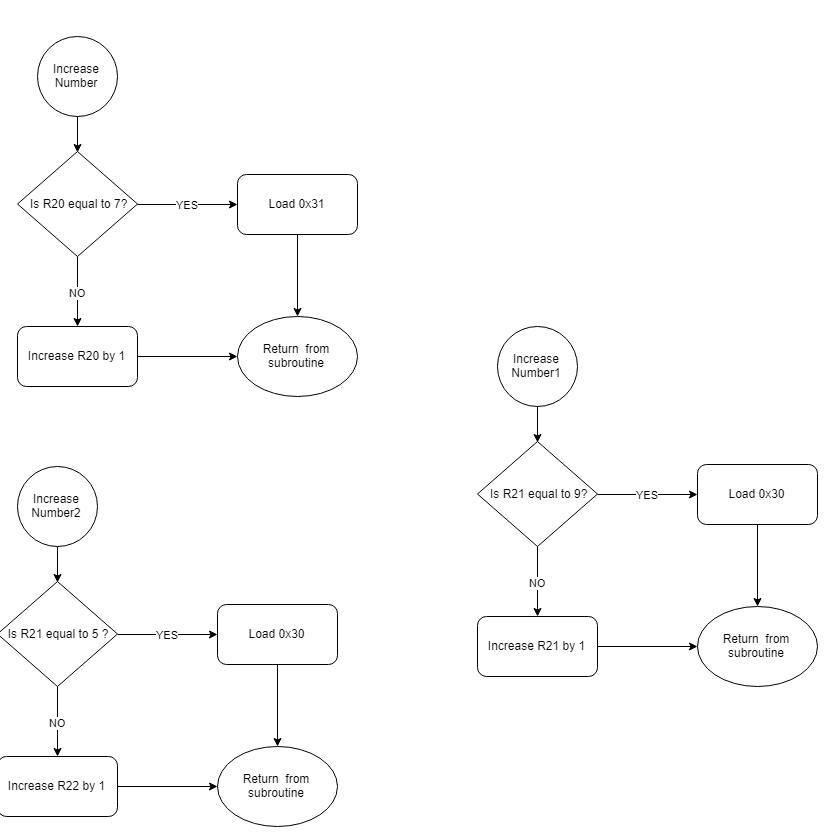
\includegraphics[scale=0.9]{img/Task2-3.png}
\end{center}
\newpage
\section{Task 3 -Serial communication and display}
\textit{Use program modules from lab 4 and write a program that receives a character on the serial port
and displays each character on the display. }

\lstset{style=Asm}
\begin{lstlisting}
;>>>>>>>>>>>>>>>>>>>>>>>>>>>>>>>>>>>>>>>>>>>>>>>>>>>>>>>>>>>
; 1DT301, Computer Technology I
; Date: 2019-10-11
; Author:
; Loic GALLAND
; Leonardo PEDRO
;
; Lab number: 5
; Title: Display JHD202
;
; Hardware: STK600, CPU ATmega2560
;
; Function: program that receives a character on the serial port and displays each character on the display. 
;
; Input ports: No input ports
;
; Output ports: PORTE for the display
;
; Subroutines: If applicable.
; Included files: m2560def.inc
;<<<<<<<<<<<<<<<<<<<<<<<<<<<<<<<<<<<<<<<<<<<<<<<<<<<<<<<<<<<
.include 	"m2560def.inc"
.def	Temp	= r16
.def	Data	= r17
.def	RS	= r18


.equ	BITMODE4	= 0b00000010		; 4-bit operation
.equ	CLEAR	= 0b00000001			; Clear display
.equ	DISPCTRL	= 0b00001111		; Display on, cursor on, blink on.

.cseg
.org	0x0000				; Reset vector
	jmp reset

.org URXC1addr	;USART Interrupt
rjmp GetChar

.org	0x0072

reset:	

	ldi Temp, HIGH(RAMEND)	; Temp = high byte of ramend address
	out SPH, Temp			; sph = Temp
	ldi Temp, LOW(RAMEND)	; Temp = low byte of ramend address
	out SPL, Temp			; spl = Temp

	ser Temp				; r16 = 0b11111111
	out DDRE, Temp			; port E = outputs ( Display JHD202A)
	clr Temp				; r16 = 0
	out PORTE, Temp	
	
	ldi r16, 23		;osc = 1.843MHz, 4800 bps => UBBRR = 23
	sts UBRR1L , r16	;Store Prescaler value in UBRR1L

	ldi r16, (1<<RXEN1 | 1<<TXEN1);Set RX, TX enable flags and RXCIE = 1
	sts UCSR1B, r16
	sei	;Set global interrupt flag

; **
; ** init_display
; **
init_disp:	
	rcall power_up_wait		; wait for display to power up
	ldi Data, BITMODE4		; 4-bit operation
	rcall write_nibble		; (in 8-bit mode)
	rcall short_wait		; wait min. 39 us
	ldi Data, DISPCTRL		; disp. on, blink on, curs. On
	rcall write_cmd			; send command
	rcall short_wait		; wait min. 39 us
	
call clr_disp

GetChar:	;Receive data
	lds r20, UCSR1A	;read UCSR1A I/0 register to r20
	sbrs r20,RXC1	;RXC1=1 -> new Character
	rjmp GetChar	;RXC1=0 -> no character received
	lds r23,UDR1	;Read character in UDR

	Port_output:
		mov Data,r23
		call write_char
	PutChar:
	lds r20, UCSR1A	;Read UCSR1A i/O register to r20
	sbrs r20, UDRE1	;UDRE1 =1 => buffer is empty 
	rjmp PutChar	;UDRE1 = 0 => buffer is not empty
	sts UDR1,r23	;write character to UDR1
rjmp GetChar	;Return to loop

clr_disp:	
	ldi Data, CLEAR			; clr display
	rcall write_cmd			; send command
	rcall long_wait			; wait min. 1.53 ms
	ret

; **
; ** write char/command
; **
write_char:		
	ldi RS, 0b00100000		; RS = high
	rjmp write
write_cmd: 	
	clr RS					; RS = low
write:	
	mov Temp, Data			; copy Data
	andi Data, 0b11110000	; mask out high nibble
	swap Data				; swap nibbles
	or Data, RS				; add register select
	rcall write_nibble		; send high nibble
	mov Data, Temp			; restore Data
	andi Data, 0b00001111	; mask out low nibble
	or Data, RS				; add register select

write_nibble:
	rcall switch_output		; Modify for display JHD202A, port E
	nop						; wait 542nS
	sbi PORTE, 5			; enable high, JHD202A
	nop
	nop						; wait 542nS
	cbi PORTE, 5			; enable low, JHD202A
	nop
	nop						; wait 542nS
	ret

; **
; ** busy_wait loop
; **
short_wait:	
	clr zh					; approx 50 us
	ldi zl, 30
	rjmp wait_loop
long_wait:	
	ldi zh, HIGH(1000)		; approx 2 ms
	ldi zl, LOW(1000)
	rjmp wait_loop
dbnc_wait:	
	ldi zh, HIGH(4600)		; approx 10 ms
	ldi zl, LOW(4600)
	rjmp wait_loop
power_up_wait:
	ldi zh, HIGH(9000)		; approx 20 ms
	ldi zl, LOW(9000)

wait_loop:	
	sbiw z, 1				; 2 cycles
	brne wait_loop			; 2 cycles
	ret

; **
; ** modify output signal to fit LCD JHD202A, connected to port E
; **
switch_output:
	push Temp
	clr Temp
	sbrc Data, 0				; D4 = 1?
	ori Temp, 0b00000100		; Set pin 2 
	sbrc Data, 1				; D5 = 1?
	ori Temp, 0b00001000		; Set pin 3 
	sbrc Data, 2				; D6 = 1?
	ori Temp, 0b00000001		; Set pin 0 
	sbrc Data, 3				; D7 = 1?
	ori Temp, 0b00000010		; Set pin 1 
	sbrc Data, 4				; E = 1?
	ori Temp, 0b00100000		; Set pin 5 
	sbrc Data, 5				; RS = 1?
	ori Temp, 0b10000000		; Set pin 7 (wrong in previous version)
	out porte, Temp
	pop Temp
	ret
\end{lstlisting}
This is the flowchart of the task 3:
\begin{center}
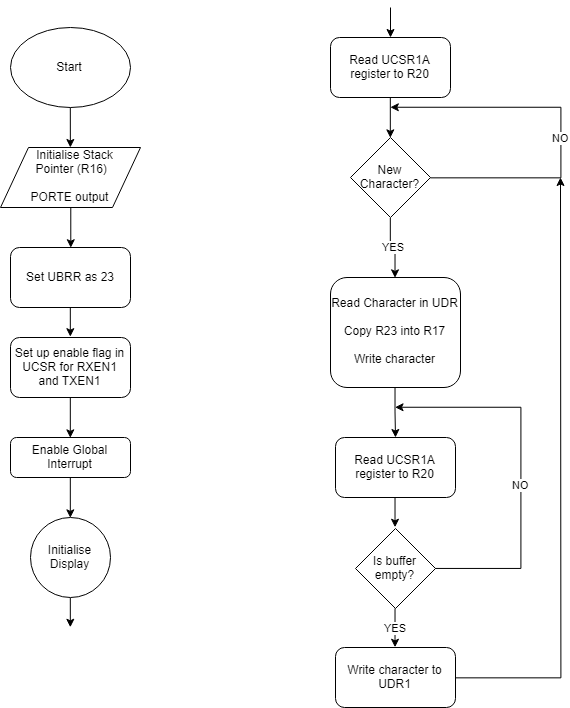
\includegraphics[scale=0.8]{img/TASK3.png}
\end{center}
\newpage
\section{Task 4 - Modify the program in task 3}
\textit{Modify the program in task 3 so that 4 lines of text can be displayed. Each textline should
be displayed during 5 seconds, after that the text on line 1 should be moved to line 2 and
so on. The text should be entered from the terminal program, PUTTY, via the serial port. }

\lstset{style=Asm}
\begin{lstlisting}
;>>>>>>>>>>>>>>>>>>>>>>>>>>>>>>>>>>>>>>>>>>>>>>>>>>>>>>>>>>>
; 1DT301, Computer Technology I
; Date: 2019-10-11
; Author:
; Loic GALLAND
; Leonardo PEDRO
;
; Lab number: 5
; Title: Display JHD202
;
; Hardware: STK600, CPU ATmega2560
;
; Function: program that receives a character on the serial port and displays each character on the display. 
;
; Input ports: No input ports
;
; Output ports: PORTE for the display
;
; Subroutines: If applicable.
; Included files: m2560def.inc
;<<<<<<<<<<<<<<<<<<<<<<<<<<<<<<<<<<<<<<<<<<<<<<<<<<<<<<<<<<<
.include 	"m2560def.inc"
.def	Temp	= r16
.def	Data	= r17
.def	RS	= r25
.def	COUNTER = r24


.equ	BITMODE4	= 0b00000010		; 4-bit operation
.equ	CLEAR	= 0b00000001			; Clear display
.equ	DISPCTRL	= 0b00001111		; Display on, cursor on, blink on.

.cseg
.org	0x0000				; Reset vector
	jmp reset

.org URXC1addr	;USART Interrupt
rjmp GetChar

.org	0x0072

reset:	
	ldi COUNTER,0
	ldi Temp, HIGH(RAMEND)	; Temp = high byte of ramend address
	out SPH, Temp			; sph = Temp
	ldi Temp, LOW(RAMEND)	; Temp = low byte of ramend address
	out SPL, Temp			; spl = Temp

	ser Temp				; r16 = 0b11111111
	out DDRE, Temp			; port E = outputs ( Display JHD202A)
	clr Temp				; r16 = 0
	out PORTE, Temp	
	
	ldi r16, 23		;osc = 1.843MHz, 4800 bps => UBBRR = 23
	sts UBRR1L , r16	;Store Prescaler value in UBRR1L

	ldi r16, (1<<RXEN1 | 1<<TXEN1);Set RX, TX enable flags and RXCIE = 1
	sts UCSR1B, r16
	sei	;Set global interrupt flag
	;Inialiaze Y and X pointer to memory address 0x200
	ldi YH , HIGH (0x200)
	ldi YL , LOW(0x200)
	ldi XH , HIGH (0x200)
	ldi XL , LOW(0x200)

; **
; ** init_display
; **
init_disp:	
	rcall power_up_wait		; wait for display to power up
	ldi Data, BITMODE4		; 4-bit operation
	rcall write_nibble		; (in 8-bit mode)
	rcall short_wait		; wait min. 39 us
	ldi Data, DISPCTRL		; disp. on, blink on, curs. On
	rcall write_cmd			; send command
	rcall short_wait		; wait min. 39 us
	
call clr_disp

GetChar:	;Receive data
	lds r21, UCSR1A	;read UCSR1A I/0 register to r20
	sbrs r21,RXC1	;RXC1=1 -> new Character
	rjmp GetChar	;RXC1=0 -> no character received
	lds r23,UDR1	;Read character in UDR
	cpi r23,0x0D
	breq next_line
	st Y+,r23

	Port_output:
		;call clr_disp
		mov Data,r23
		call write_char
	PutChar:
	lds r21, UCSR1A	;Read UCSR1A i/O register to r20
	sbrs r21, UDRE1	;UDRE1 =1 => buffer is empty 
	rjmp PutChar	;UDRE1 = 0 => buffer is not empty
	sts UDR1,r23	;write character to UDR1
	rjmp END

	next_line:
		rcall FiveSec_delay
		ldi Data, CLEAR
		rcall write_cmd
		rcall long_wait
		ldi Data, 0x40
		rcall write_cmd
		;clr Data

			loop:
			;COMPARARE BEFORE IT GETS MEMORY OUT OF BOUNDARY
				cp YH , XH
				brne continue_printing
				cp YL , XL
				breq Stop
			
				continue_printing:
					ld Data,X+	;load from X pointer to Data
					rcall write_char
					rcall long_wait
				rjmp loop

			Stop:		;Reinialize the pointers 
				ldi YH , HIGH (0x200)
				ldi YL , LOW(0x200)
				ldi XH , HIGH (0x200)
				ldi XL , LOW(0x200)
				ldi Data, 0b00000010
				rcall write_cmd
		
			rjmp End
END:nop
rjmp GetChar	;Return to loop


clr_disp:	
	ldi Data, CLEAR			; clr display
	rcall write_cmd			; send command
	rcall long_wait			; wait min. 1.53 ms
	ret

; **
; ** write char/command
; **

write_char:		
	ldi RS, 0b00100000		; RS = high
	rjmp write
write_cmd: 	
	clr RS					; RS = low
write:	
	mov Temp, Data			; copy Data
	andi Data, 0b11110000	; mask out high nibble
	swap Data				; swap nibbles
	or Data, RS				; add register select
	rcall write_nibble		; send high nibble
	mov Data, Temp			; restore Data
	andi Data, 0b00001111	; mask out low nibble
	or Data, RS				; add register select

write_nibble:
	rcall switch_output		; Modify for display JHD202A, port E
	nop						; wait 542nS
	sbi PORTE, 5			; enable high, JHD202A
	nop
	nop						; wait 542nS
	cbi PORTE, 5			; enable low, JHD202A
	nop
	nop						; wait 542nS
	ret

; **
; ** busy_wait loop
; **
short_wait:	
	clr zh					; approx 50 us
	ldi zl, 30
	rjmp wait_loop
long_wait:	
	ldi zh, HIGH(1000)		; approx 2 ms
	ldi zl, LOW(1000)
	rjmp wait_loop
dbnc_wait:	
	ldi zh, HIGH(4600)		; approx 10 ms
	ldi zl, LOW(4600)
	rjmp wait_loop
power_up_wait:
	ldi zh, HIGH(9000)		; approx 20 ms
	ldi zl, LOW(9000)

wait_loop:	
	sbiw z, 1				; 2 cycles
	brne wait_loop			; 2 cycles
	ret

FiveSec_delay:
; Generated by delay loop calculator
; at http://www.bretmulvey.com/avrdelay.html
; Delay 9 215 000 cycles
; 5s at 1.843 MHz
    ldi  r18, 47
    ldi  r19, 192
    ldi  r20, 104
L1: dec  r20
    brne L1
    dec  r19
    brne L1
    dec  r18
    brne L1
RET

; **
; ** modify output signal to fit LCD JHD202A, connected to port E
; **
switch_output:
	push Temp
	clr Temp
	sbrc Data, 0				; D4 = 1?
	ori Temp, 0b00000100		; Set pin 2 
	sbrc Data, 1				; D5 = 1?
	ori Temp, 0b00001000		; Set pin 3 
	sbrc Data, 2				; D6 = 1?
	ori Temp, 0b00000001		; Set pin 0 
	sbrc Data, 3				; D7 = 1?
	ori Temp, 0b00000010		; Set pin 1 
	sbrc Data, 4				; E = 1?
	ori Temp, 0b00100000		; Set pin 5 
	sbrc Data, 5				; RS = 1?
	ori Temp, 0b10000000		; Set pin 7 (wrong in previous version)
	out porte, Temp
	pop Temp
	ret
\end{lstlisting}

\newpage
This is the flowchart of the task 4:
\begin{center}
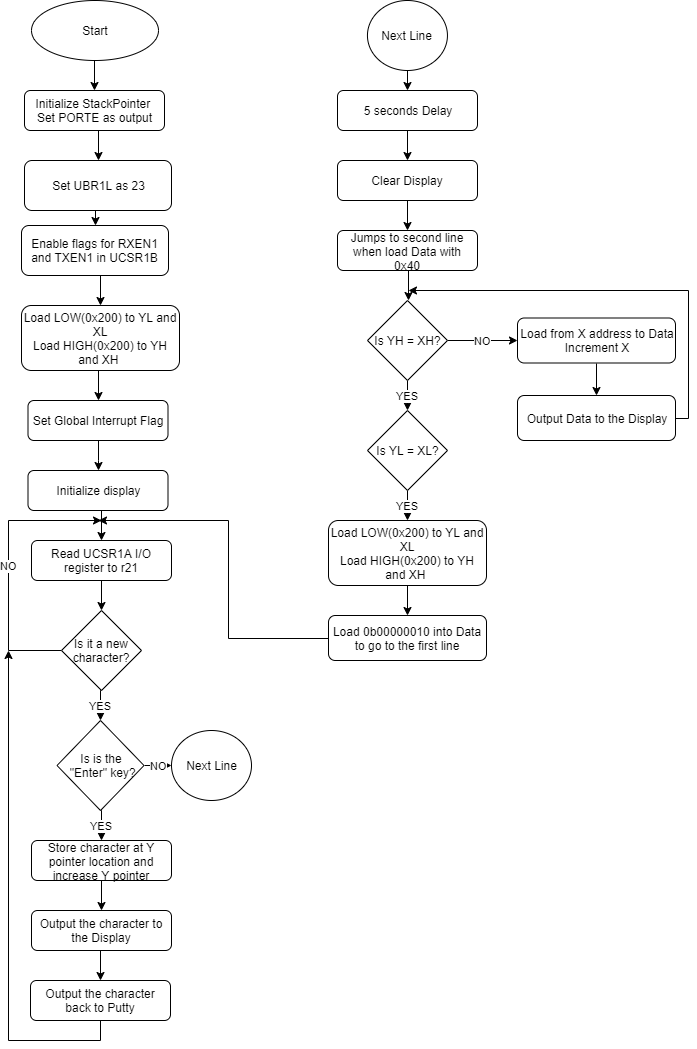
\includegraphics[scale=0.6]{img/Task4.png}
\end{center}
% Prints your bibliography database xxx.bib
\bibliographystyle{IEEEtran}
\bibliography{ref.bib}

\end{document}
